\documentclass[mathserif]{beamer}

\usetheme{Boadilla}
\usecolortheme{dolphin}

\setbeamertemplate{navigation symbols}{} 
\setbeamertemplate{footline}{}
%\setbeamercovered{transparent}

\setbeamertemplate{title page} {
    \begin{center}
    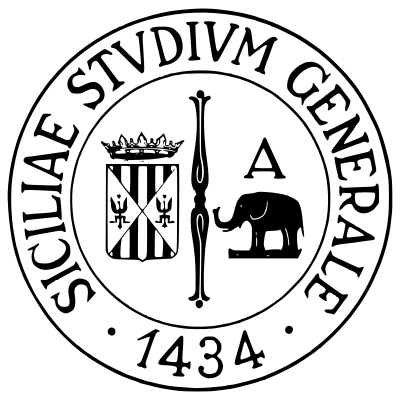
\includegraphics[width=0.15\textwidth]{img/unict.png} \\
    \small{
        \insertinstitute
    } \\
    \vskip0.02\textwidth
    \hrule
    \vskip2em
    \begin{beamercolorbox}[center,shadow=true,rounded=true]{title}
    {\LARGE{\inserttitle}}
    \vskip2pt
    \end{beamercolorbox}
    \begin{center}
    \Large{\textbf{\insertauthor}}\\
    \end{center}
    \vskip2em
    \vfill
    \insertdate
    \end{center}
}

\defbeamertemplate*{footline}{my theme}
{
  \leavevmode%
  \hbox{%
  \begin{beamercolorbox}[wd=.40\paperwidth,ht=2.25ex,dp=1ex,center]{author in head/foot}%
    \usebeamerfont{author in head/foot}\insertshortauthor~~(\insertshortinstitute)
  \end{beamercolorbox}%
  \begin{beamercolorbox}[wd=.40\paperwidth,ht=2.25ex,dp=1ex,center]{title in head/foot}%
    \usebeamerfont{title in head/foot}\insertshorttitle
  \end{beamercolorbox}%
  \begin{beamercolorbox}[wd=.20\paperwidth,ht=2.25ex,dp=1ex,right]{date in head/foot}%
    \usebeamerfont{date in head/foot}\insertshortdate{}\hspace*{2em}
    \insertframenumber{}\hspace*{2ex} 
  \end{beamercolorbox}}%
  \vskip0pt%
}


% Spaces
\newcommand{\N}{\vskip 0.4 cm}
\newcommand{\n}{\vskip 0.2 cm}
\newcommand{\TAB}{\hskip 4 cm}
\newcommand{\tab}{\hskip 0.6 cm}

%Vector notation
\newcommand{\vectornorm}[1]{\left|\left|#1\right|\right|}

% Colors
\newcommand{\red}[1]{\textcolor[rgb]{.8,0,0}{#1}}
\newcommand{\blue}[1]{\textcolor[rgb]{0,0,.7}{#1}}
\newcommand{\navy}[1]{\textcolor[rgb]{0,0,.5}{#1}}
\newcommand{\purple}[1]{\textcolor[rgb]{.7,0,.8}{#1}}
\newcommand{\green}[1]{\textcolor[rgb]{0,.6,.1}{#1}}


\title[Darpooling]
{Darpooling\\* A Distributed Carpooling system}
\subtitle{A distributed graph analysis with WS}
\author[A. Lima - D. Marletta]{Antonio Lima e Daniele Marletta}
\institute[UniCT]{
    Universit\`a degli Studi di Catania\\
        CdL in Ingegneria Informatica - Laurea Specialistica \\
        Corso di Sistemi Distribuiti
}
\date[29/09/2010]{29 September 2010}


\begin{document}

%------------------------------TITLE Pages
%\begin{frame}[label=t,plain]
\begin{frame}[plain]
  \titlepage
\end{frame}
%

\section{Introduction}

\begin{frame}{Carpooling}  
\begin{quote}
Carpooling is the sharing of car journeys so that more than one person travels in a car.

\flushright{
    \footnotesize{
    \color{blue}
        \url{http://en.wikipedia.org/wiki/Carpool}
    }
}
\end{quote}

\vfill

Carpooling lets reduce negative aspects of private transportation: costs,
traffic, pollution, parking spaces crowd. It is also a good way to socialize and meet new people.
Reliability of arrangements can be increased with use of trusting metrics
in the carpooling management system.
\end{frame}

\begin{frame}{A Carpooling software}

The main challenge of this work is to ensure scalability: 
it should be easy to add/remove/modify management servers. Other challenges
such as security, efficiency, reliability, ... are not meant to be
addressed here.
\vfill

\textbf{Architecture proposed}
\begin{itemize}
\item
Management servers connected in a P2P network (over the Internet)
\item
Each client accesses a server through Internet or a local network 
(Bluetooth, wifi, Zigbee, ...)
\item
The client can use global system services, regardless of which server it is
connected to.
\end{itemize}
\end{frame}

\begin{frame}[plain]
\begin{center}
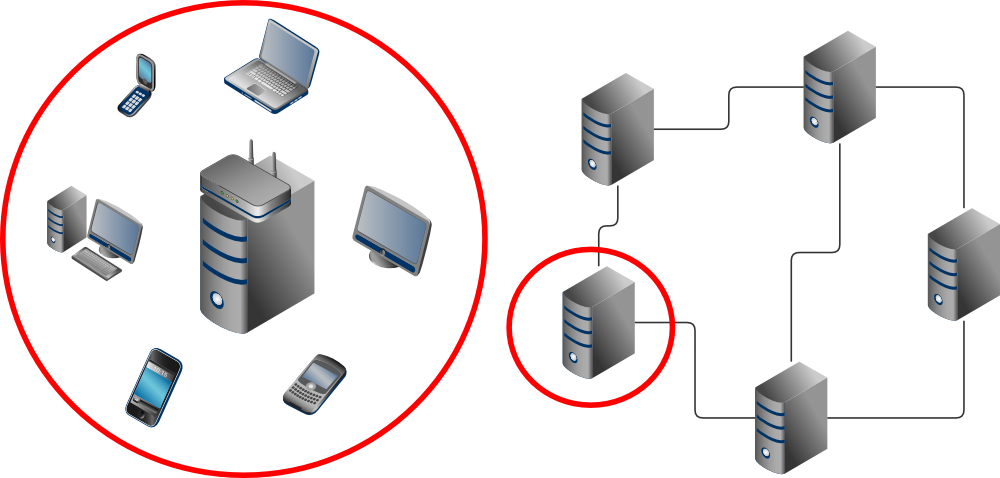
\includegraphics[width=0.95\textwidth]{img/darpooling.png}
\end{center}
\end{frame}

\end{document}
